\section{Physics motivation\label{sec:physHI}}
\label{sec:physics}

{\bf [Yen-Jie working on this section]}

In this Section we discuss the physics performance of the upgraded L1 trigger system for the 2018 high luminosity PbPb run using three examples of measurements using rare probes. 
The performance of the upgraded system, which uses background subtraction for L1 event rejection and provides 
access to the full expected luminosity of 3~nb$^{-1}$ is compared to that of the current system. 
These examples illustrate the large improvements in statistical precision afforded by the  improved 
ability to select jet events and high \pt\ particles during high luminosity PbPb collisions. 


%Studies of high \pt\ jet and charged particle production in the 2010 and 2011 PbPb data sets have helped to elucidate the nature of parton energy loss in hot nuclear matter. Parton energy loss was characterized using a wide range 
%of different signatures, ranging from the the dijet energy imbalance in central collisions and the suppression of single particle
%spectra at the highest \pt\ to modifications of jet shapes and fragmentation patterns~\cite{Chatrchyan:2011sx,Aamodt:2010jd,Alice:dihadron,CMS:2012aa,Chatrchyan:2012nia,Aad:2010bu,atlas:2012is,Chatrchyan:2012gt,Chatrchyan:2012gw}. 

Below we discuss a selection of measurements which exploit the future high luminosity data sets to 
provide important insights into the parton energy loss mechanism and heavy flavor particle production:

\begin{enumerate}
\item The flavor dependence of jet quenching is a crucial important test ground for various parton energy loss models. 
Compared to light quarks, heavy quarks are expected to suffer from smaller radiative energy loss when passing 
through the medium because gluon radiation is suppressed at angles smaller than the ratio of the quark mass $M$ to 
its energy $E$~\cite{Dokshitzer:2001zm}. This effect (and its disappearance at high \pt) can be studied using tagging
of b-decays and b-jets.
\item Compared to quarks, gluons are expected to suffer a larger 
energy loss because of the larger color factors. This effect can be studied using three-jet events.
\item Measurements of the single particle azimuthal anisotropy at very high \pt\ give access to the in-medium path-length 
dependence of energy loss. The azimuthal anisotropy as a function of charged particle \pt\ also yields 
important information about the parton energy dependence of the energy loss. 
\item Jet-heavy flavor meson correlation
\end{enumerate}


These and other measurements rely on a sufficiently selective jet and heavy flavor meson trigger to provide access to the 
full delivered luminosity and a large minimum-bias sample.  Data collected during the 2015 PbPb run were used to estimate physics reach  
for a future high-luminosity run (assuming $L_{int} =$3~nb$^{-1}$) for these three physics cases. 
%Using typical thresholds of leading jet \pt\ $>100$~GeV/c, Figure~\ref{fig:efficiency_comparison} shows that 
%with the upgraded system (labeled ``Stage-1 system'' in the plots) sufficient rejection factors can be 
%achieved to sample the full delivered luminosity. For the current system (labeled ``Current system'' in the 
%plots), the rejection factor at L1 is limited to about two, requiring a large prescale factor to be applied
%due to bandwidth constraints in the detector front end readout. Figure~\ref{fig:aj_2015} to 
%\ref{fig:xT_scaling} show the effect of the resulting difference in statistical reach 
%for the physics examples discussed below.

\begin{figure}[!ht]
\begin{center}
%\includegraphics[width=.60\textwidth]{fig/heavyIon//efficiency_comparison_l1primitives.pdf}
\caption{The jet finder is applied to minimum bias data from 2011 without
event selection using the L1 primitives present in the RAW data. The
fraction of events which have a jet above a given $E_t$ threshold is plotted
as a function of that threshold. Note that the threshold is applied to the
L1 jet energy and does not correspond to the HLT or offline jet energy
scales.}
\label{fig:efficiency_comparison}
\end{center}
\end{figure}


\subsection{Nuclear Modification Factors of Heavy Flavor Mesons}
{\bf [To be updated]}

One of the proposed observables that reveal the flavor dependence of in-medium parton energy loss is the reduction of heavy flavor meson yield. This can be studied by measurements of nuclear modification factors ($R_{AA}$), defined as the ratio of the yield in nucleus-nucleus collisions to that observed in pp collisions, scaled by the number of binary nucleon-nucleon collisions. Examples of theoretcal calculations of $R_{AA}$ for D and B mesons are shown in Figure~\ref{fig:RAA_theory}. At low pT, the production rate of heavy flavor meson in PbPb is sensitive to the elastic energy loss of the heavy quark, gluon shadowing and the recombination of the heavy quark and light flavors. At high pT, the size of the suppression is sensitive to the heavy quark radiative energy loss in the pQCD based models and has a chance to tell us about the pathlength dependence of the heavy quark energy loss (ads/cft vs pQCD). Precise measurement of the heavy flavor meson production from low pt to high pt will provide important constrain to the physical effect mentioned before.

\begin{figure}[!ht]
\begin{center}
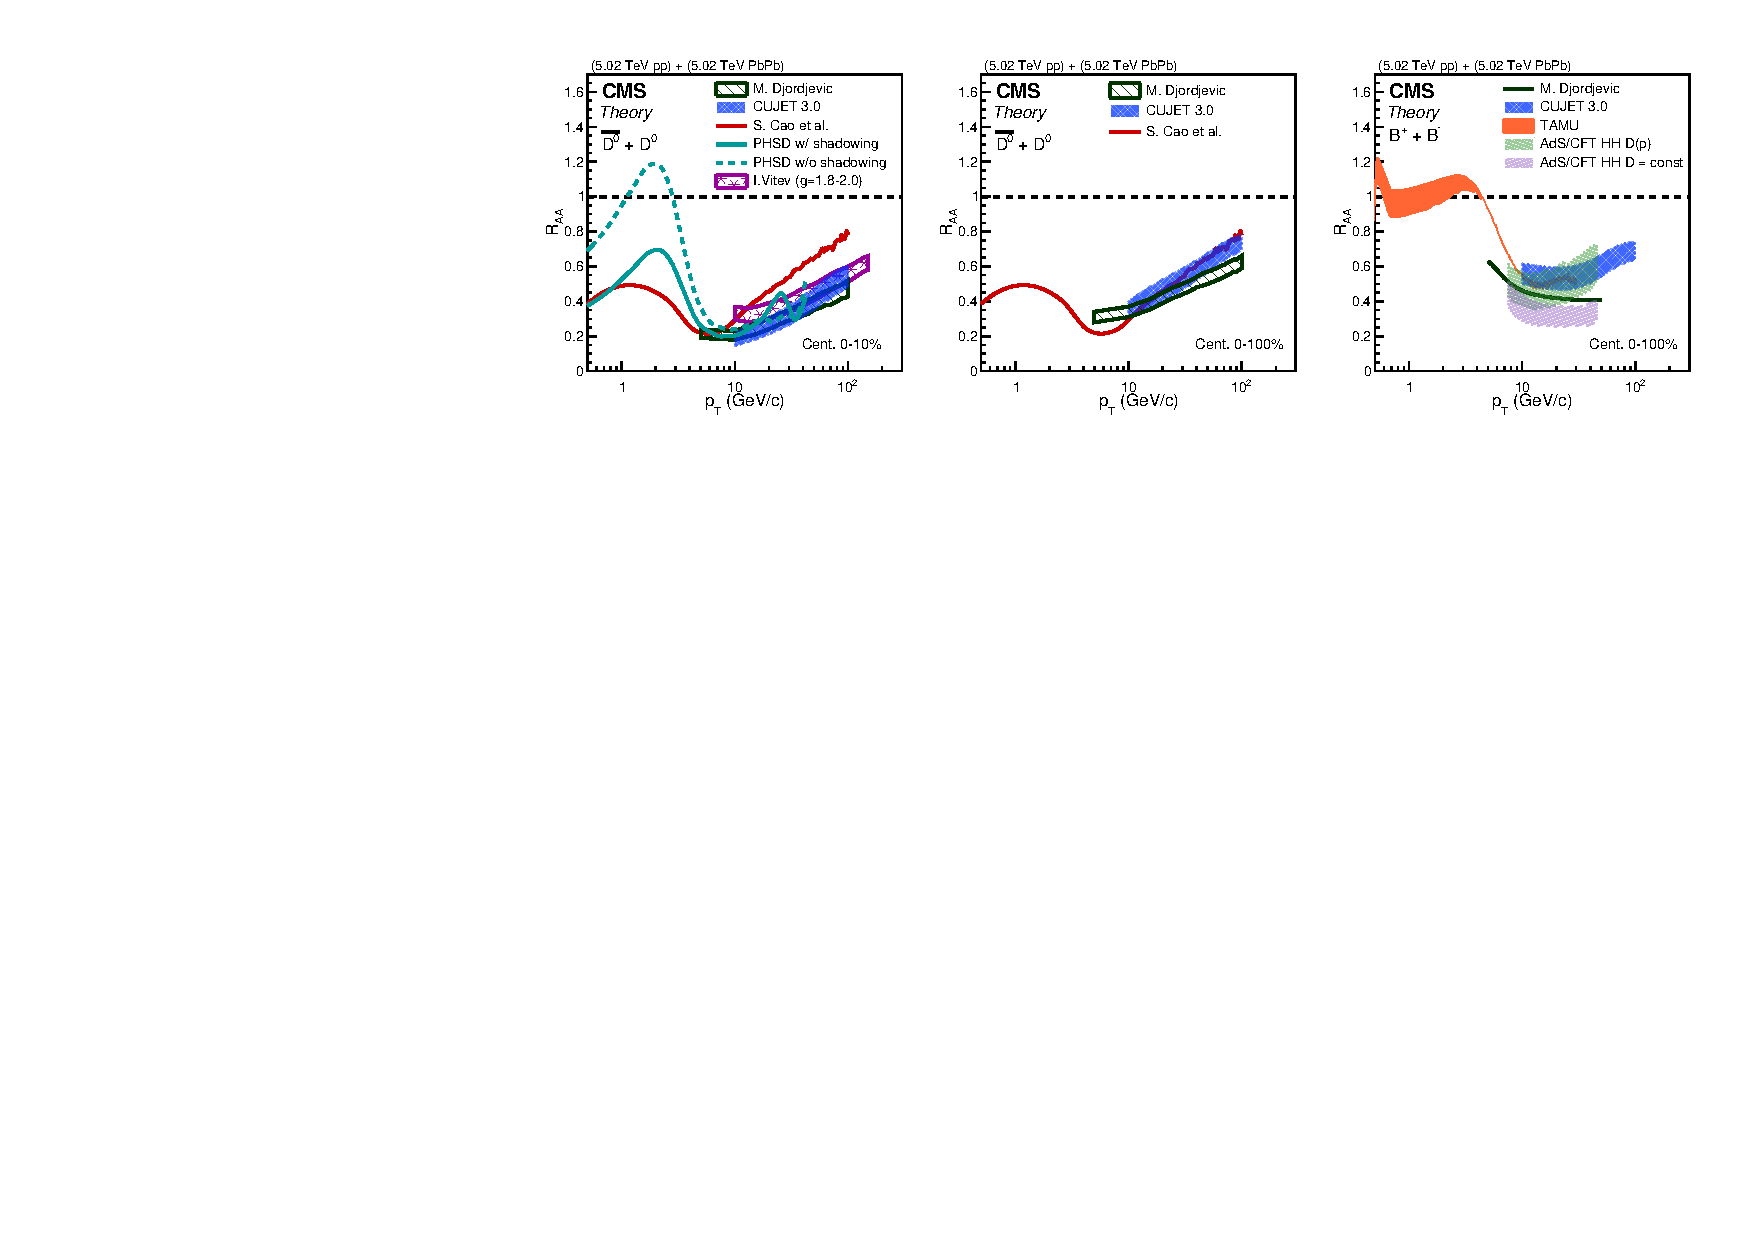
\includegraphics[width=.90\textwidth]{figures/cTheoryRAA_BD_v1.pdf}
\caption{Theoretical calculations of nuclear modification factors of charged particles, $D^0$ and $B^+$ mesons.}
\label{fig:RAA_theory}
\end{center}
\end{figure}

In order to study the recombination of the heavy quark and light flavor, comparison between the RAA from $D^0$ ($B^+$), $D_s$ ($B_s$) and $\Lambda_c$ ($\Lambda_b$) gives us important insights. Due to the larger strangeness content in the QGP, $D_s$ ($B_s$) are expected to be relatively less suppressed compared to $D^0$ ($B^+$) in the recombination models. Figure~\ref{fig:HFMesonMass} shows the proof of principle studies of $D_s$ and $\Lambda_c$ in the heavy ion collisions with the CMS detector, projected to the expected statistics to be collected with the L1 trigger rate upgrade. Significant signals of Ds and $\Lambda_c$ could be observed which enable the measurement of Ds and $\Lambda_c$ RAA for the first time. 


\begin{figure}[!ht]
\begin{center}
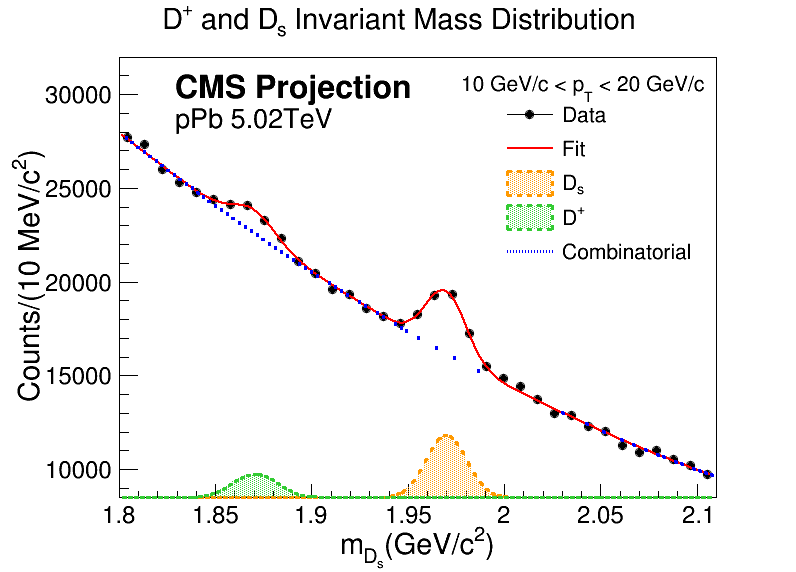
\includegraphics[width=.45\textwidth]{InvMassFigures/Ds.png}
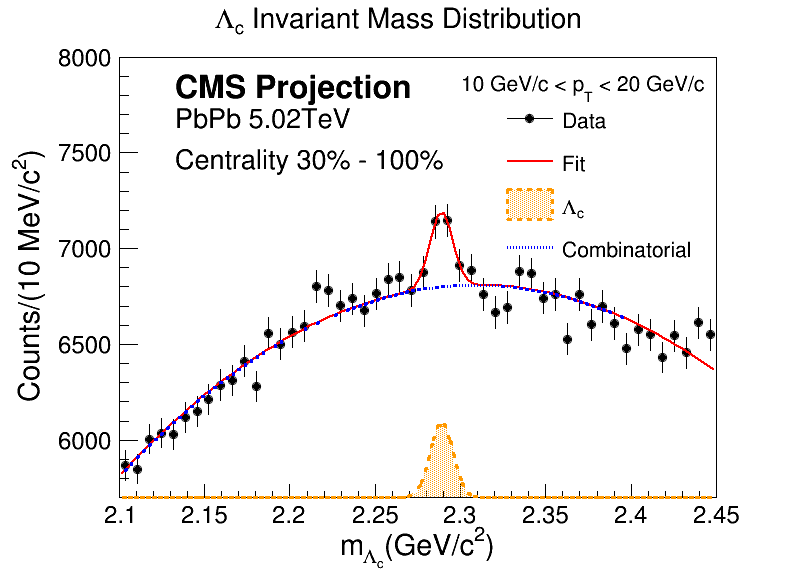
\includegraphics[width=.45\textwidth]{InvMassFigures/LambdaC.png}
\caption{Invariant mass distributions}
\label{fig:HFMesonMass}
\end{center}
\end{figure}

Figure~\ref{} shows the expected performance with the data recorded in 2015 and the projected performance in 2018 and beyond. With the high statistics jet and heavy flavor triggered sample, the precision of the RAA measurements at high pT could be greatly improved. At the same time, with the L1 trigger rate upgrade proposed in this proposal, the large minimum-bias sample enable the CMS collaboration to perform the studies down to very low pT region. The expected precision of $D^0$, $B^+$ and $D_s$ $R_{AA}$ measurements from low pT to high pT could provide strong constrain on the theoretical models and the difference in the suppression magnitude between those mesons could be observed for the first time.


\begin{figure}[!ht]
\begin{center}
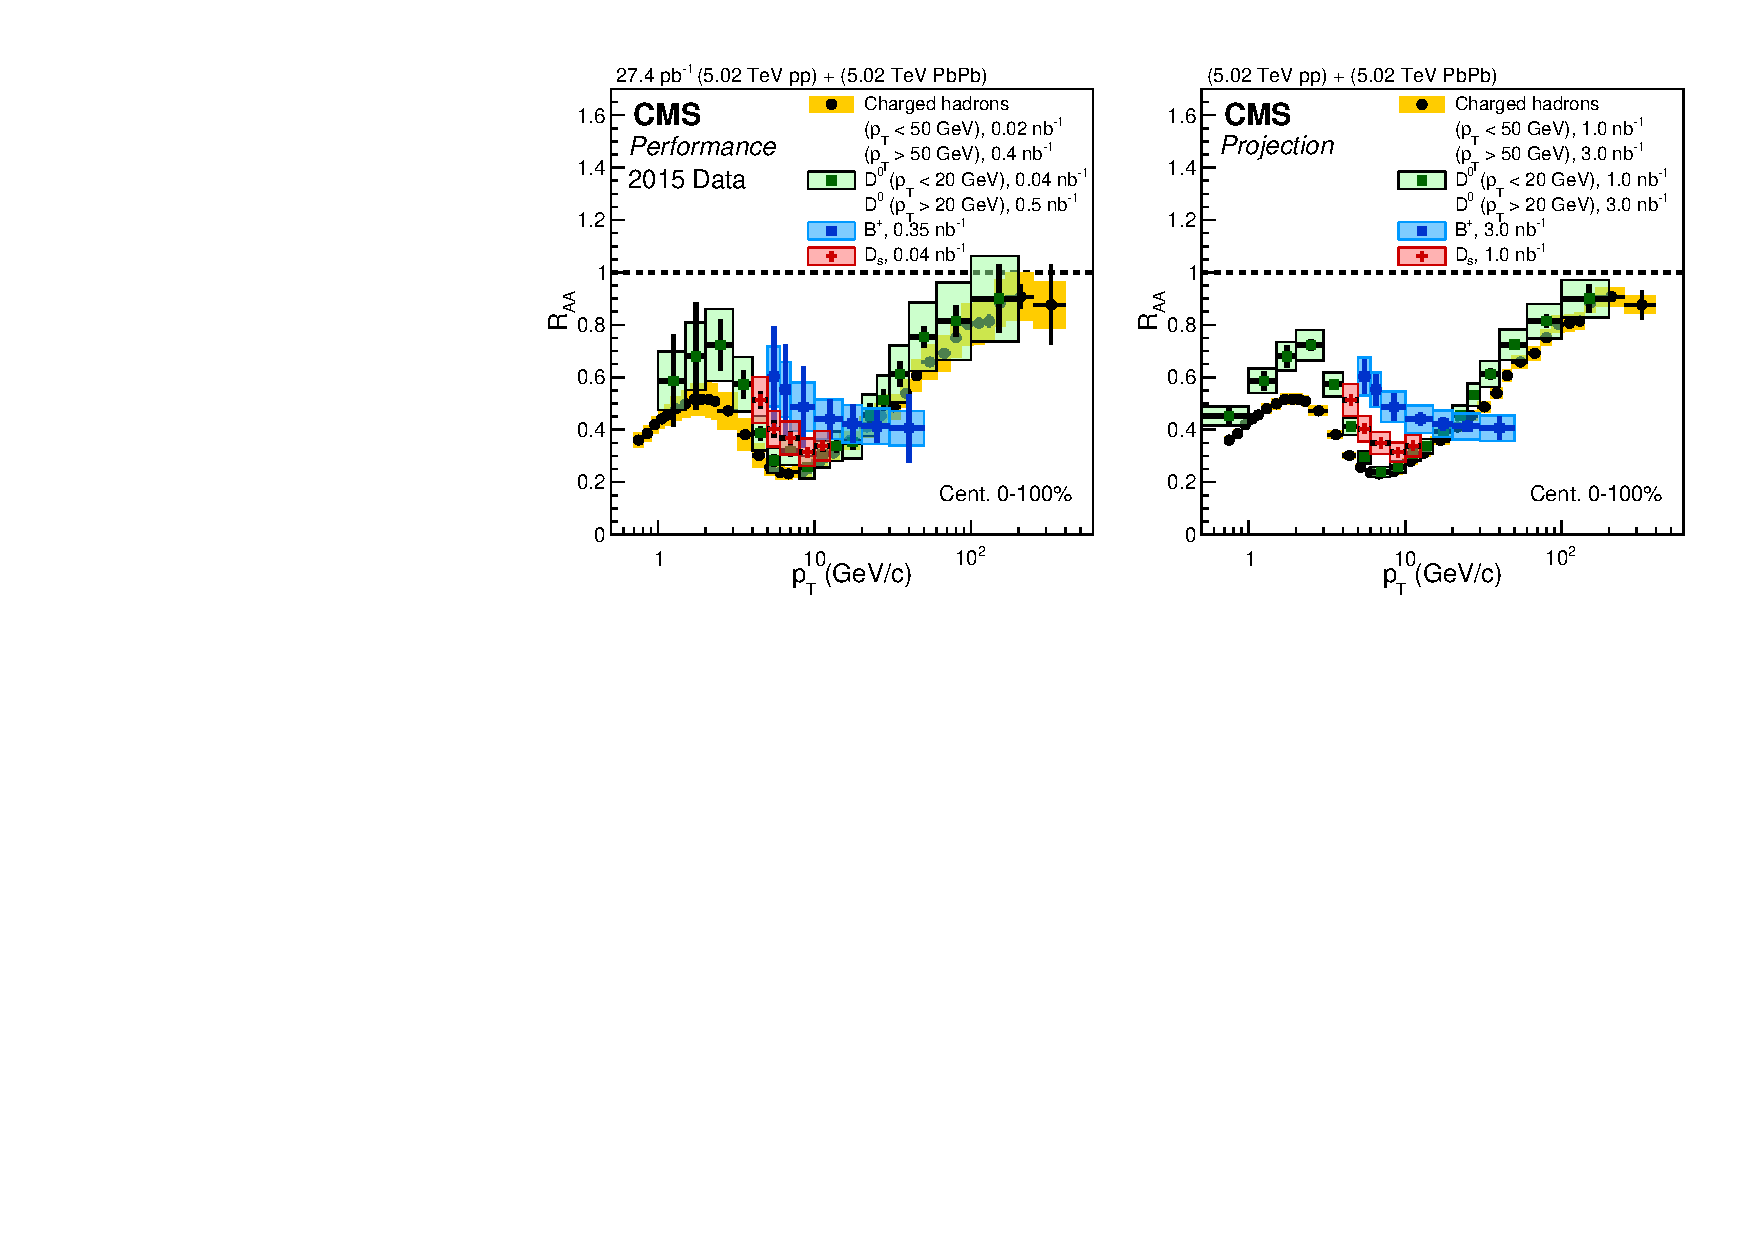
\includegraphics[width=.90\textwidth]{figures/cRAA_lumiTG_3_lumiMB_1_v2.pdf}
\caption{Nuclear modification factors of charged particles, $D^0$, $D_s$ and $B^+$ mesons with 2015 data (left panel) and the statistics expected with L1 trigger rate upgrade.}
\label{fig:RAA_2015}
\end{center}
\end{figure}

\subsection{Ellipic Flow of Heavy Flavor Mesons}

The expected precision of the elliptic flow ($v_2$) measurements of the charged particle, $D^0$ and $D_s$ mesons are shown in Figure~\ref{fig:v2_projection}.

\begin{figure}[!ht]
\begin{center}
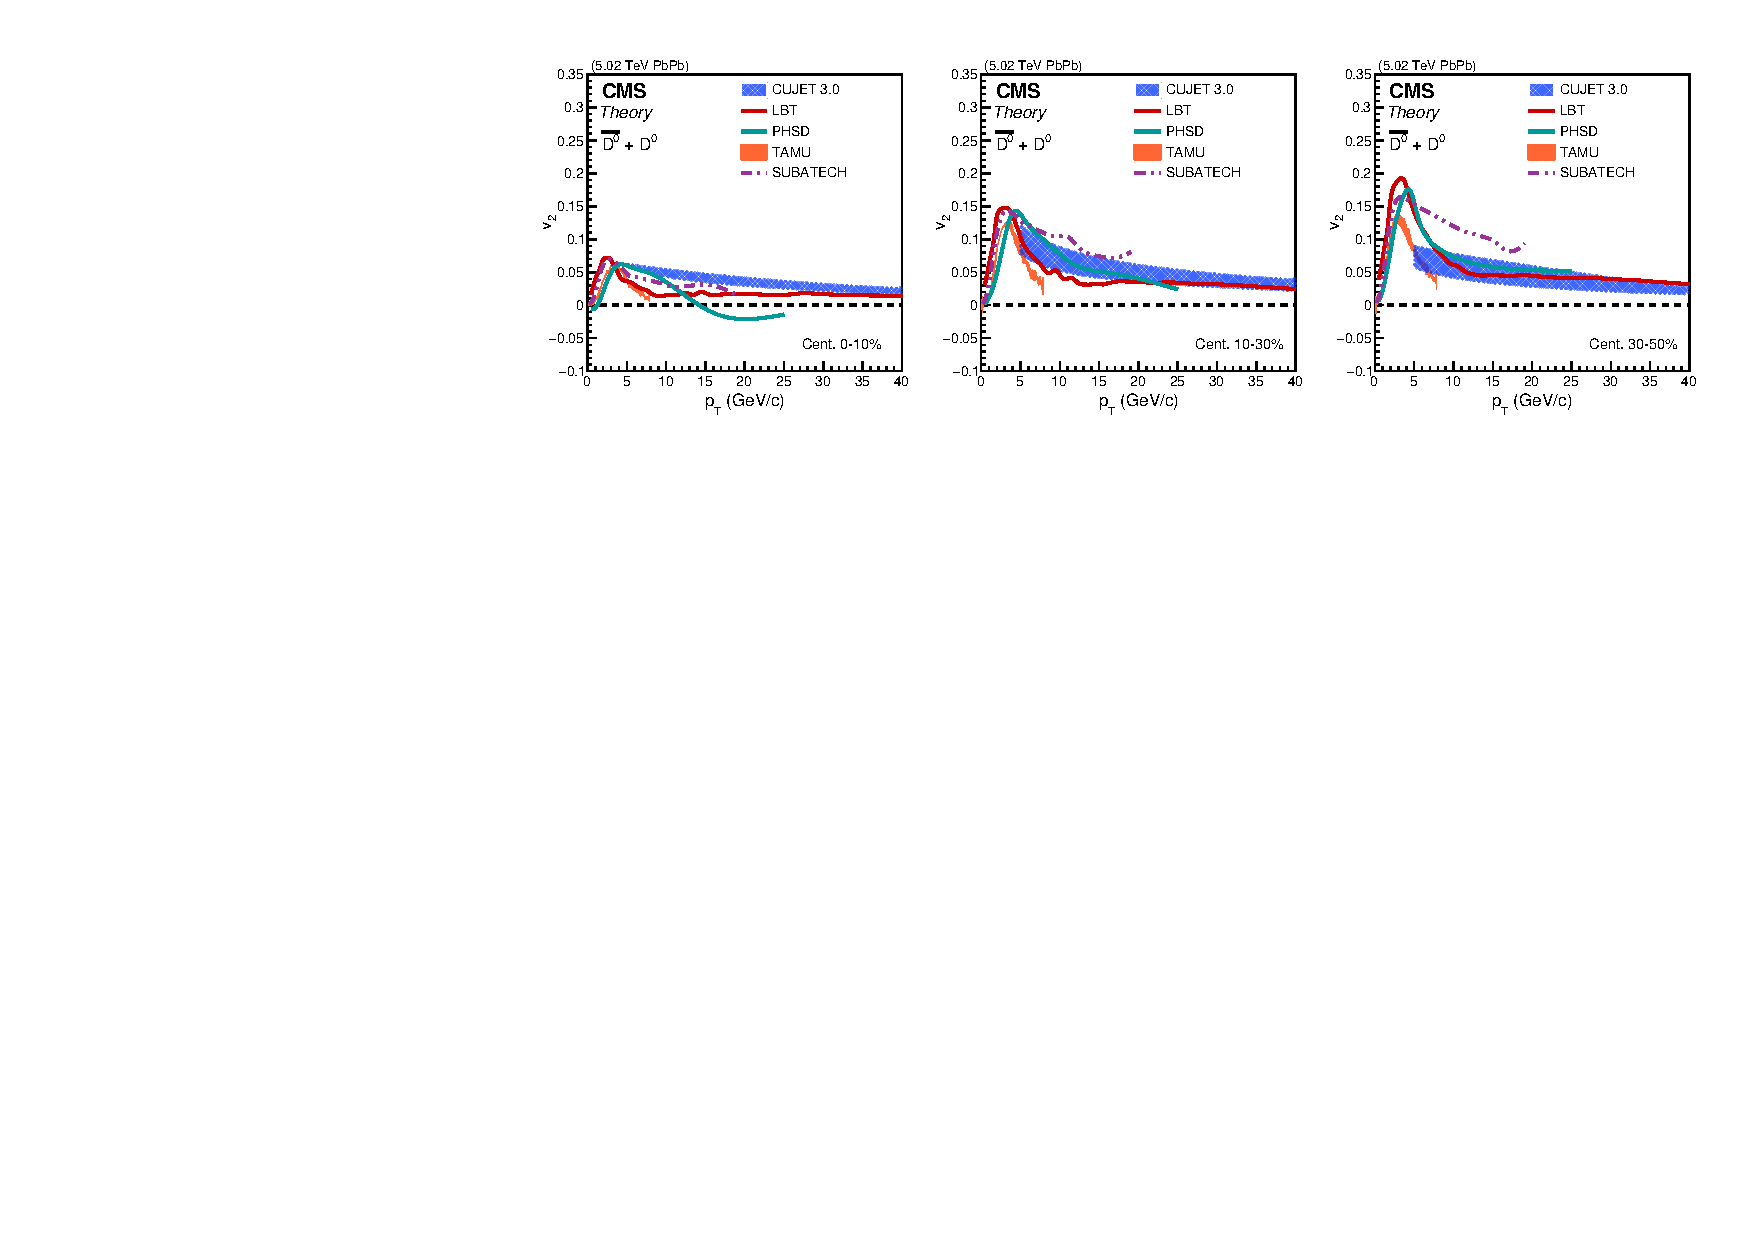
\includegraphics[width=.90\textwidth]{figures/cTheoryV2_D_v1.pdf}
\caption{Theoretical calculations of v2.}
\label{fig:v2_theory}
\end{center}
\end{figure}

\begin{figure}[!ht]
\begin{center}
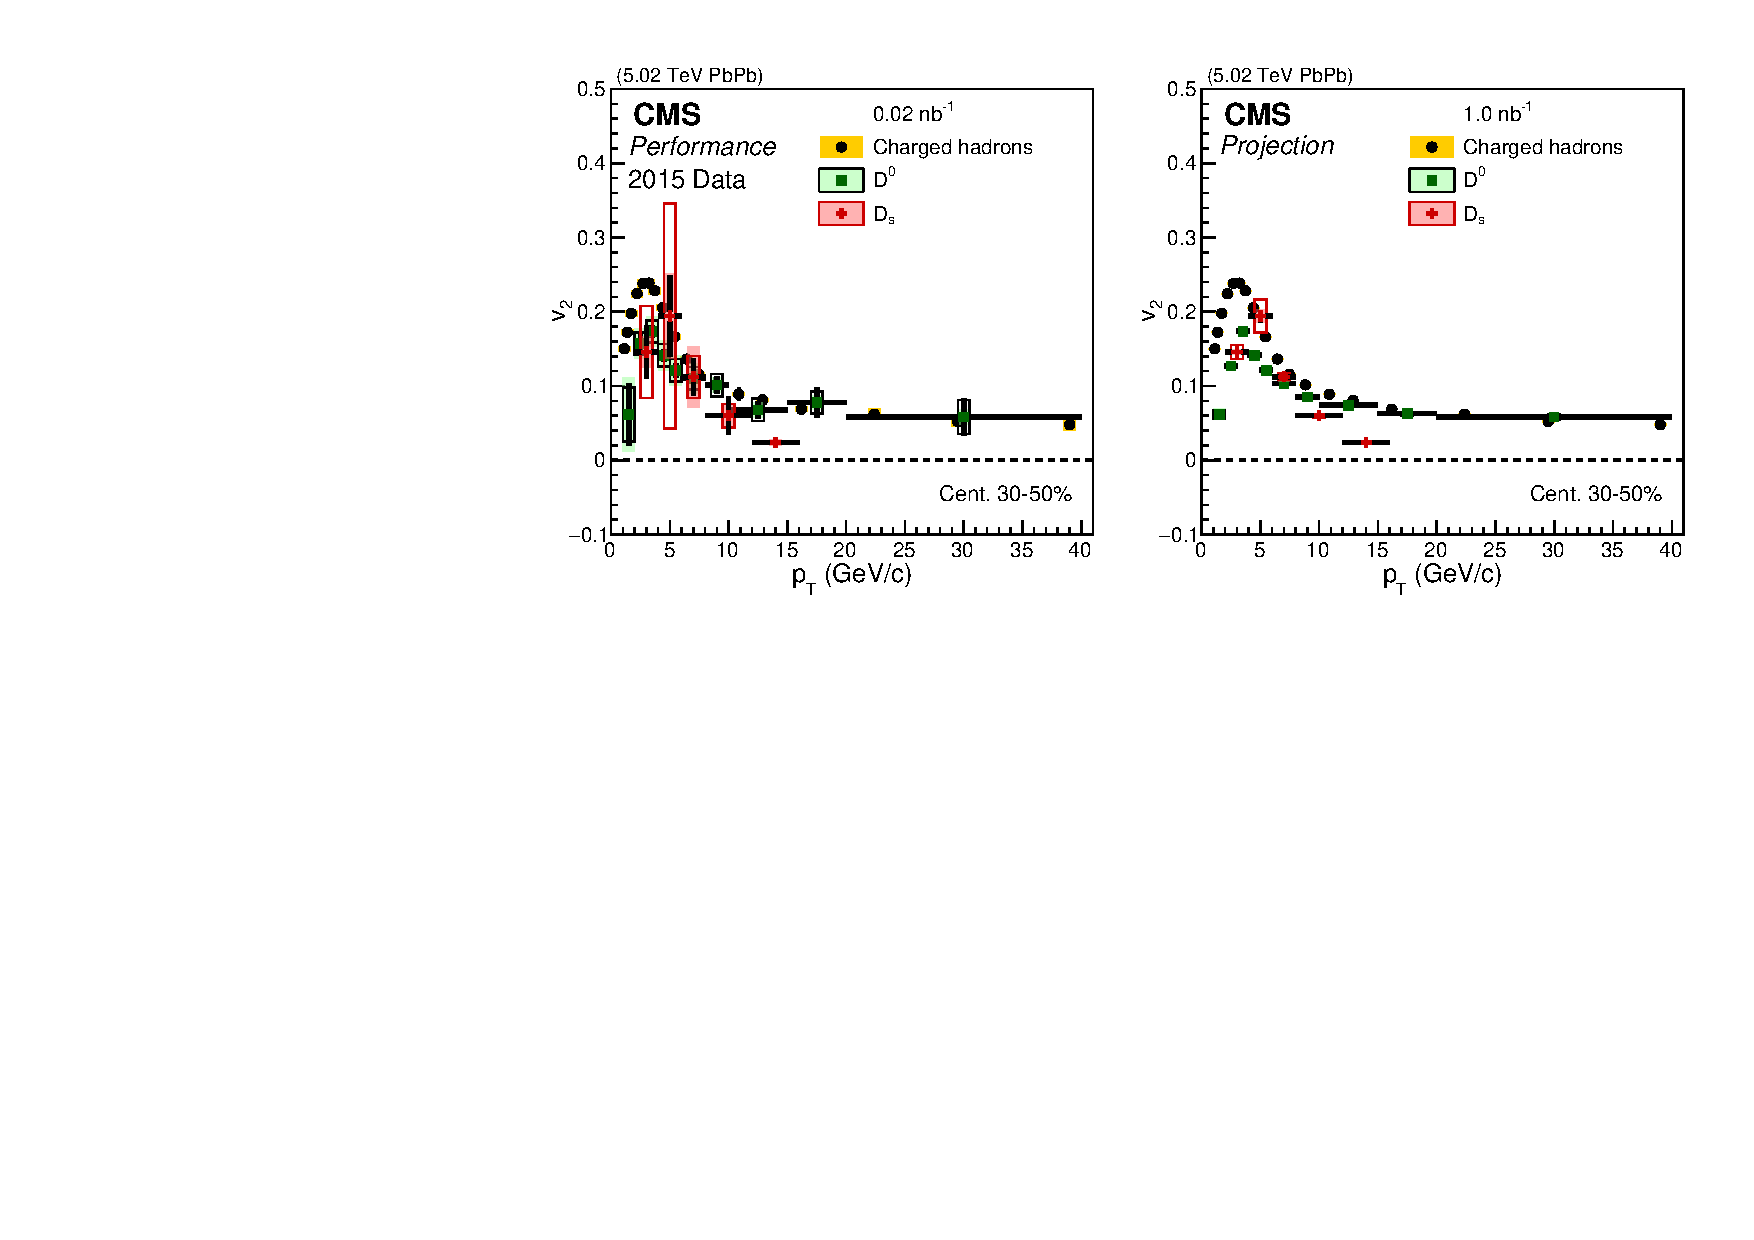
\includegraphics[width=.90\textwidth]{figures/cV2_lumiMB_1.pdf}
\caption{V2 measurement.}
\label{fig:v2_projection}
\end{center}
\end{figure}



\subsection{$D^0$-Jet and $D^0$-hadron correlations}

Studies of $D^0$-jet and $D^0$-hadron angular correlation are sensitive to energy loss mechanism. 


\subsection{Summary}

\begin{table}[hbt]
\begin{center}
\begin{tabular}{ |c|c|c|c|c| } 



\cline{1-5}
\multicolumn{5}{|c|}{\textbf{Measurements of Current Pixel System and 2018 Pixel System} }\\
 \cline{1-5}
     &   \multicolumn{2}{p{6cm}|}{ \textbf{Current 0.04 $nb^{-1}$ + Legacy Pixel System}}  & \multicolumn{2}{p{6cm}|} {\textbf{2018 PbPb 1 $nb^{-1}$ + Pixel Upgrade}} \\
            \cline{1-5}
\hline
Observables & $p_T$ min & Statistical Uncertainty & $p_T$ min & Statistical Uncertainty  \\
\hline
$D^0 R_{AA}$ & 2 & 15\% & 0.5 - 1 & 10\% \\
\hline
$D_s R_{AA}$ & $\sim$ 4 & 20\% & $<$ 4  & 4\% \\
\hline
$\Lambda_c R_{AA}$ & 10 & $>$ 20\% & $<$ 10 & 4\% \\
\hline
$B \rightarrow D R_{AA}$ & 6 & 20\% & 2 & 10\% \\
\hline
$B^+ (D^0 \pi) R_{AA}$ & Not accessible & & $\sim$ 4 & \\
\hline
Low $p_T $ c and b jets & Not accessible &  &  & \\
\hline
$D^0 v_2$ (= 0.06) & 1 & 80\% & 0.5 - 1 & 18\% \\
\hline
$D_s v_2$ & Not accessible &  & $\sim$ 4 &  \\
\hline
$B \rightarrow D v_2$ & Not accessible &  & $\sim$ 2 &  \\
\hline
$\Lambda_c v_2$ & Not accessible &  & $\sim$ 6 &  \\
\hline

\end{tabular}
\end{center}
\caption{Summary of the heavy flavor measurements with 2015 data and 2018 data with L1 trigger rate upgrade}
\label{OpCost}
\end{table}

\clearpage

